% =========================================================================
% --- INICIO INPUT SEMANA 3 ---
% =========================================================================

\chapter{Semana 3: Shift de Bernoulli y Semi-Conjugación}

\section{Shift de Bernoulli}

Sea $X = \{z_1, z_2, \dots, z_d\}$ un alfabeto finito equipado con la topología discreta generada por la métrica $d_1: X \times X \to \mathbb{R}^+_0$:
$$d_1(u, v) = \begin{cases} 0 & u = v \\ 1 & u \neq v \end{cases}$$
Definimos los espacios de sucesiones:
\begin{itemize}
	\item El espacio unilateral: $\Sigma^+ = X^{\mathbb{N}} = \{(x_n)_{n \in \mathbb{N}} : x_n \in X\}$
	\item El espacio bilateral: $\Sigma = X^{\mathbb{Z}} = \{(x_n)_{n \in \mathbb{Z}} : x_n \in X\}$
\end{itemize}

Podemos dotar a estos espacios de la siguiente métrica (escrita para $\Sigma$, de forma análoga para $\Sigma^+$):
$$d((x_n)_{n \in \mathbb{Z}}, (y_n)_{n \in \mathbb{Z}}) = \sum_{n \in \mathbb{Z}} \frac{d_1(x_n, y_n)}{2^{|n|}}$$

\begin{proposicion}
	La función $d$ es una métrica en $\Sigma$ (y en $\Sigma^+$).
\end{proposicion}
\begin{proof}
	Claramente está bien definida (converge), pues:
	$$ \sum_{n \in \mathbb{Z}} \frac{d_1(x_n, y_n)}{2^{|n|}} = \sum_{n \in \mathbb{N}} \frac{d_1(x_n, y_n)}{2^n} + \frac{d_1(x_0, y_0)}{2^0} + \sum_{n \in \mathbb{N}} \frac{d_1(x_{-n}, y_{-n})}{2^{-n}} \le \sum_{n \in \mathbb{N}} \frac{1}{2^n} + 1 + \sum_{n \in \mathbb{N}} \frac{1}{2^n} < 1 + 1 + 1 = 3 $$
	Los resultados siguientes son obvios porque $d_1$ es una métrica:
	\begin{enumerate}[i)]
		\item Si $(x_n)_{n \in \mathbb{Z}} = (y_n)_{n \in \mathbb{Z}} \implies \forall n \in \mathbb{Z} \implies x_n = y_n, \forall n \in \mathbb{Z} \implies d_1(x_n, y_n) = 0 \implies d((x_n), (y_n)) = 0$.
		Si $d((x_n), (y_n)) = 0 \implies d_1(x_n, y_n) = 0, \forall n \in \mathbb{Z} \implies x_n = y_n, \forall n \in \mathbb{Z} \implies (x_n) = (y_n)$.
		\item $d((x_n), (y_n)) = \sum_{n \in \mathbb{Z}} \frac{d_1(x_n, y_n)}{2^{|n|}} = \sum_{n \in \mathbb{Z}} \frac{d_1(y_n, x_n)}{2^{|n|}} = d((y_n), (x_n))$.
		\item Sea $(x_n), (y_n), (z_n) \in \Sigma \implies d((x_n), (y_n)) = \sum_{n \in \mathbb{Z}} \frac{d_1(x_n, y_n)}{2^{|n|}} \le \sum_{n \in \mathbb{Z}} \frac{d_1(x_n, z_n) + d_1(z_n, y_n)}{2^{|n|}} = d((x_n), (z_n)) + d((z_n), (y_n))$.
	\end{enumerate}
\end{proof}

\begin{definicion}[Cilindros]
	Un \textbf{cilindro} de longitud $k$ es el conjunto de todas las sucesiones que tienen símbolos fijos en coordenadas específicas. Lo denotamos por:
	$$[n_1: c_1, \dots, n_k: c_k] = \{(x_n) \in \Sigma : x_{n_i} = c_i \text{ para } i=1,\dots,k\}$$
\end{definicion}

\begin{observacion}
	Sea $X = \{z_1, z_2, \dots, z_d\}$ un conjunto finito y $\Sigma = X^{\mathbb{Z}}$.
	\begin{enumerate}[a)]
		\item $\Sigma = \bigsqcup_{i=1}^d [j: z_i]$ con $j \in \mathbb{Z}$ arbitrario y fijo.
		\item $\Sigma = \bigsqcup_{i,m=1}^d [j: z_i, z_m]$ con $j \in \mathbb{Z}$ arbitrario y fijo.
	\end{enumerate}
	En $X$ estamos considerando la topología generada por $d_1$. Así, $X$ es un espacio topológico compacto (Ejercicio).
	Como $\Sigma = X^{\mathbb{Z}}$ (y $\Sigma^+ = X^{\mathbb{N}}$), podemos considerar la topología producto en $\Sigma$, lo cual garantiza por el Teorema de Tychonoff que $\Sigma$ es compacto.
\end{observacion}

\begin{ejercicio}
	Mostrar que la colección de cilindros en $\Sigma^+$ (o en $\Sigma$) es una base topológica para la topología en $\Sigma^+$ (o en $\Sigma$) generada por $d$.
\end{ejercicio}
\begin{proof}[Solución]
	Sea $B = B_\epsilon((x_n)_{n \in \mathbb{Z}})$ con $\epsilon > 0$ y $(y_n)_{n \in \mathbb{Z}} \in B$. Sea $\delta = \min\{d(x,y), \epsilon - d(x,y)\}$. 
	Como $\delta > 0$, dividimos con un número $K \in \mathbb{N}$ tal que $0 < \delta/K = \delta^* < 1$, donde $K \ge 3$.
	Como $\delta^* < 1 \implies \exists n_0 \in \mathbb{N} / \frac{1}{2^{n_0-1}} = \sum_{n=n_0+1}^\infty \frac{1}{2^{n-1}} < \delta^*$. 
	Luego, definimos el cilindro: $C = [-n_0 : y_{-n_0}, \dots, n_0 : y_{n_0}]$. Claramente $(y_n)_{n \in \mathbb{N}} \in C$.
	
	Sea $(z_n)_{n \in \mathbb{Z}} \in C \implies d((z_n), (y_n)) = \sum_{n \in \mathbb{Z}} \frac{d_1(z_n, y_n)}{2^{|n|}} + \sum_{n \in \mathbb{N}} \frac{d_1(z_{-n}, y_{-n})}{2^n} = \sum_{n=n_0+1}^\infty \frac{d_1(z_n, y_n)}{2^n} + \sum_{n=n_0+1}^\infty \frac{d_1(z_{-n}, y_{-n})}{2^n} \le 2 \sum_{n=n_0+1}^\infty \frac{1}{2^n} < 2\delta^* < \delta$.
	Luego, $(z_n)_{n \in \mathbb{Z}} \in B_\delta(y) \implies (z_n)_{n \in \mathbb{Z}} \in C \subseteq B$.
\end{proof}

\begin{figure}[htbp]
	\centering
	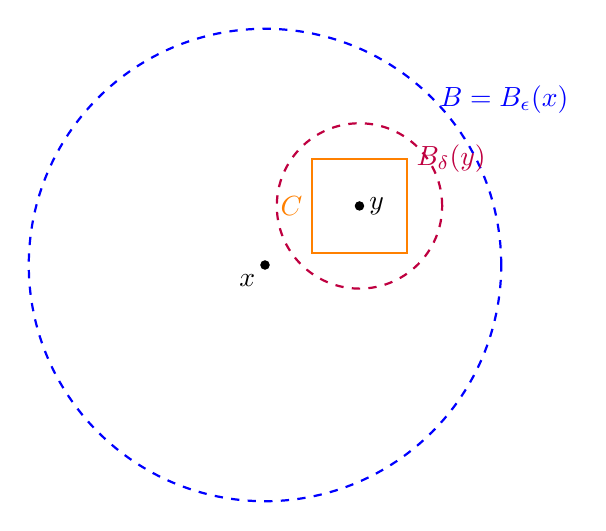
\begin{tikzpicture}[scale=1.5]
		% Bola grande B (alrededor de x)
		\draw[blue, thick, dashed] (0,0) circle (2cm);
		\node[blue, right] at (1.4, 1.4) {$B = B_\epsilon(x)$};
		\filldraw[black] (0,0) circle (1pt) node[below left] {$x$};
		
		% Bola pequeña B_delta (alrededor de y)
		\draw[purple, thick, dashed] (0.8,0.5) circle (0.7cm);
		\node[purple, right] at (1.2, 0.9) {$B_\delta(y)$};
		\filldraw[black] (0.8,0.5) circle (1pt) node[right] {$y$};
		
		% Cilindro C (alrededor de y)
		\draw[orange, thick] (0.4, 0.1) rectangle (1.2, 0.9);
		\node[orange, left] at (0.4, 0.5) {$C$};
	\end{tikzpicture}
	\caption{El cilindro $C$ está contenido en la vecindad $B_\delta(y)$, la cual a su vez está contenida en el abierto original $B$.}
\end{figure}

\begin{ejercicio}
	Mostrar que cualquier cilindro $[m: a_m, \dots, a_n]$ es un conjunto abierto en $\Sigma^+$ (o en $\Sigma$) con la topología en $\Sigma^+$ (o en $\Sigma$) generada por $d$.
\end{ejercicio}
\begin{proof}[Solución]
	Sea $C = [m: a_m, \dots, a_n]$ un cilindro. Sea $x = (x_k) \in C$. 
	Queremos encontrar un $\epsilon > 0$ tal que $B_\epsilon(x) \subseteq C$. 
	Basta tomar $\epsilon < \frac{1}{2^{\max(|m|, |n|)}}$. Sea $y = (y_k) \in B_\epsilon(x)$, entonces $d(x, y) < \epsilon$.
	Si existiera algún $k \in [m, n]$ tal que $y_k \neq x_k = a_k$, entonces $d_1(x_k, y_k) = 1$.
	Esto implicaría que $d(x, y) \ge \frac{d_1(x_k, y_k)}{2^{|k|}} = \frac{1}{2^{|k|}} \ge \frac{1}{2^{\max(|m|, |n|)}} > \epsilon$, lo cual es una contradicción ($\rightarrow \leftarrow$).
	Por ende, $y_k = a_k$ para todo $k \in [m, n]$, lo que implica que $y \in C$. Así, $B_\epsilon(x) \subseteq C$, demostrando que el cilindro es un conjunto abierto.
\end{proof}

\begin{ejercicio}
	Mostrar que la topología en $\Sigma^+$ (en $\Sigma$) generada por $d$ es igual a la topología producto $\tau$.
\end{ejercicio}
\begin{proof}[Solución]
	i) Sea $U$ abierto en la topología producto: $U = B_{\epsilon_{i_1}} \times \dots \times B_{\epsilon_{i_n}} \times \prod_{j \neq i_1,\dots,i_n} X$, donde $\epsilon_{i_1}, \dots, \epsilon_{i_n} > 0$. Donde $j \in \mathbb{Z}$.
	Donde $x = (x_n)_{n \in \mathbb{Z}} \in U$. Definimos $C = [i_1: x_{i_1}, \dots, i_n: x_{i_n}]$. Luego, $x \in C \subseteq U$.
	
	ii) La forma análoga es muy sencilla. 
	Como la topología generada por $d$ es equivalente a la que es generada por cilindros, entonces es equivalente a la topología producto.
\end{proof}

\begin{definicion}[Shift de Bernoulli]
	Sea $X = \{z_1, \dots, z_d\}$, $\Sigma^+ = \{(x_n)_{n \in \mathbb{N}} : x_n \in X\}$ y $\Sigma = \{(x_n)_{n \in \mathbb{Z}} : x_n \in X\}$. Definimos:
	\begin{itemize}
		\item \textbf{Shift Unilateral:} $\sigma: \Sigma^+ \to \Sigma^+$ dado por $(x_n)_{n \in \mathbb{N}} \mapsto \sigma((x_n)_{n \in \mathbb{N}}) = (y_n)_{n \in \mathbb{N}}$, donde $y_n = x_{n+1}, \forall n \in \mathbb{N}$.
		\item \textbf{Shift Bilateral:} $\sigma: \Sigma \to \Sigma$ dado por $(x_n)_{n \in \mathbb{Z}} \mapsto \sigma((x_n)_{n \in \mathbb{Z}}) = (y_n)_{n \in \mathbb{Z}}$, donde $y_n = x_{n+1}, \forall n \in \mathbb{Z}$.
	\end{itemize}
\end{definicion}

\begin{ejemplo}
	Para el shift unilateral: Sea $X=\{0,1,2,3\}$, $\Sigma^+ = X^{\mathbb{N}}$.
	Si $(x_n)_{n \in \mathbb{N}} = (3,1,0,2,3,1,0,2,3,1,0,2,\dots) \implies (y_n)_{n \in \mathbb{N}} = \sigma((x_n)_{n \in \mathbb{N}}) = (1,0,2,3,1,0,2,3,1,0,2,\dots)$.
\end{ejemplo}

\begin{proposicion}
	El shift unilateral $\sigma: \Sigma^+ \to \Sigma^+$ cumple lo siguiente:
	\begin{enumerate}
		\item \textbf{Es continua.} En efecto, como los cilindros son los abiertos básicos en $\Sigma^+$, entonces es suficiente mostrar que $\sigma^{-1}([m: a_m, \dots, a_n])$ sea abierto en $\Sigma^+$.
		Observemos que $\sigma^{-1}([m: a_m, \dots, a_n]) = [m+1: a_m, \dots, a_n]$ pues, si $(z_n)_{n \in \mathbb{N}} \in \sigma^{-1}([m: a_m, \dots, a_n])$ entonces $(y_n) = \sigma((z_n)_{n \in \mathbb{N}}) \in [m: a_m, \dots, a_n]$.
		$y_m = a_m, y_{m+1} = a_{m+1}, \dots, y_n = a_n$.
		Como $y_k = z_{k+1} \implies z_{m+1} = a_m, z_{m+2} = a_{m+1}, \dots, z_{n+1} = a_n \implies ((z_n))_{n \in \mathbb{N}} \in [m+1: a_m, \dots, a_n]$.
		\item \textbf{No es inyectivo.} En efecto, $X = \{z_1, \dots, z_d\}$ y $\Sigma^+ = \{(x_n)_{n \in \mathbb{N}} : x_n \in X\}$. Sean $(x_n) = (z_1, z_1, z_2, z_2, z_2, \dots)$ y $(y_n) = (z_2, z_1, z_2, z_2, z_2, \dots)$.
		Vemos que $(x_n) \neq (y_n)$, pero $\sigma((x_n)) = (z_1, z_2, z_2, \dots) = \sigma((y_n))$.
		\item \textbf{Es sobre.} Para cualquier $(y_n)_{n \in \mathbb{N}} \in \Sigma^+$, consideremos $(x_n) = (z_1, y_0, y_1, \dots)$. Evidentemente $\sigma((x_n)) = (y_n)$, garantizando la sobreyectividad.
	\end{enumerate}
\end{proposicion}

\begin{ejercicio}
	Mostrar que el shift bilateral $\sigma: \Sigma \to \Sigma$ es un homeomorfismo.
\end{ejercicio}
\begin{proof}[Solución]
	\begin{itemize}
		\item \textbf{Inyectiva:} Sean $x = (x_n)_{n \in \mathbb{Z}}, y = (y_n)_{n \in \mathbb{Z}} \in \Sigma / \sigma(x) = \sigma(y) \implies (a_n)_{n \in \mathbb{Z}} = (b_n)_{n \in \mathbb{Z}}$ donde $a_n = x_{n+1} \land b_n = y_{n+1}, \forall n \in \mathbb{Z} \implies x_{n+1} = y_{n+1}, \forall n \in \mathbb{Z} \implies x = y$.
		\item \textbf{Sobre:} Sea $y = (y_n)_{n \in \mathbb{Z}} \implies \exists (x_n)_{n \in \mathbb{Z}} / x_n = y_{n-1}, \forall n \in \mathbb{Z} \implies \sigma((x_n)_{n \in \mathbb{Z}}) = (z_n)_{n \in \mathbb{Z}} / z_n = x_{n+1} = y_n, \forall n \in \mathbb{Z} \implies \sigma((x_n)) = (y_n)_{n \in \mathbb{Z}}$.
		(La inversa se define como $\sigma^{-1}: \Sigma \to \Sigma, \sigma^{-1}((x_n)_{n \in \mathbb{Z}}) = (y_n)_{n \in \mathbb{Z}} / y_n = x_{n-1}, \forall n \in \mathbb{Z}$).
		\item \textbf{Continua:} $\sigma: \Sigma \to \Sigma, \sigma^{-1}: \Sigma \to \Sigma$. Sea $C = [m: a_m, \dots, a_n]$ cualquier cilindro. $\sigma^{-1}(C) = [m+1: a_m, \dots, a_n] \land (\sigma^{-1})^{-1}(C) = \sigma(C) = [m-1: a_m, \dots, a_n]$ cilindros.
	\end{itemize}
\end{proof}

\begin{proposicion}
	Para el shift bilateral, $\overline{Per(\sigma)} = \Sigma$.
\end{proposicion}
\begin{proof}
	Como los abiertos básicos de $\Sigma$ son los cilindros, entonces es suficiente mostrar que $Per(\sigma) \cap [m: a_m, \dots, a_n] \neq \emptyset$.
	Consideremos: $(x_n)_{n \in \mathbb{Z}} = (\dots a_m \dots a_n \dots a_m \dots a_n \dots) \in [m: a_m, \dots, a_n]$ (bloque central de tamaño $n-m+1$) y evidentemente $\sigma^{n-m+1}((x_n)_{n \in \mathbb{Z}}) = (x_n)_{n \in \mathbb{Z}}$.
\end{proof}

\begin{ejercicio}
	¿Se cumple $\overline{Per(\sigma^+)} = \Sigma^+$?
\end{ejercicio}
\begin{proof}[Solución]
	Sea $x = (x_n)_{n \in \mathbb{N}} \in \Sigma^+ \land C = [m: x_m, \dots, x_r]$ con $m \ge 1$. Definimos: $y = (y_n)_{n \in \mathbb{N}} / y_{n+r} = y_n, \forall n \in \mathbb{N}$. Luego: $\sigma^r(y) = y \implies y \in Per(\sigma^+)$. Además $y \in C$, con $y_m = x_m, \dots, y_r = x_r$. Luego: $\overline{Per(\sigma^+)} = \Sigma^+$.
\end{proof}

\begin{proposicion}
	El shift bilateral $\sigma: \Sigma \to \Sigma$ es topológicamente mixing.
\end{proposicion}
\begin{proof}
	Sean $U, V \subseteq \Sigma$ abiertos en $\Sigma$ como los cilindros son los abiertos básicos de $\Sigma$, entonces existen $[p: a_p, \dots, a_q] \subseteq U, [r: b_r, \dots, b_s] \subseteq V$.
	Afirmación: $\exists n_0 \in \mathbb{N} / \sigma^n([p: a_p, \dots, a_q]) \cap [r: b_r, \dots, b_s] \neq \emptyset, \forall n \ge n_0$. Así $\sigma^n([p: a_p, \dots, a_q]) \cap [r: b_r, \dots, b_s] \subseteq \sigma^n(U) \cap V \neq \emptyset, \forall n \ge n_0$.
	Prueba de la afirmación: Existe $m \in \mathbb{N}$ y $\alpha_{-m}, \dots, \alpha_m, \beta_{-m}, \dots, \beta_m \in X$ tal que:
	$$ C_1^m = [-m: \alpha_{-m}, \dots, \alpha_m] \subseteq [p: a_p, \dots, a_q] $$
	$$ C_2^m = [-m: \beta_{-m}, \dots, \beta_m] \subseteq [r: b_r, \dots, b_s] $$
	¡Ejercicio! (Basta tomar $m = \max\{|p|, |q|, |r|, |s|\}$).
	
	Afirmación 1: Tomando $n_0 = 2m+2$. Se tiene que $\sigma^n(C_1^m) \cap C_2^m \neq \emptyset, \forall n \ge n_0$. En efecto, para cada $n = 2m+1+k, k \in \mathbb{Z}^+$ definimos $(w_i)_{i \in \mathbb{Z}}$:
	$w_i = \alpha_i$ para $|i| \le m$, y $w_i = \beta_{i-n}$ para $i = m+k+1, \dots, 3m+k+1$.
	Luego: $(w_i)_{i \in \mathbb{Z}} \in C_1^m \implies \sigma^{2m+1+k}((w_i)_{i \in \mathbb{Z}}) \in C_2^m \implies \sigma^n(C_1^m) \cap C_2^m \neq \emptyset$. Como $k$ fue arbitrario en $\mathbb{Z}^+ \implies \sigma^n(C_1^m) \cap C_2^m \neq \emptyset, \forall n \ge n_0 = 2m+2$.
\end{proof}

\begin{corolario}
	$\sigma: \Sigma \to \Sigma$ es topológicamente transitivo. (Pues $\Sigma$ es métrico, compacto separable y localmente compacto).
\end{corolario}

\section{Semi-Conjugación Topológica}

\begin{definicion}[Semi-Conjugación]
	Sean $X, Y$ espacios topológicos y $f: X \to X$, $g: Y \to Y$ aplicaciones continuas. Decimos que $g$ es un \textbf{factor} de $f$ (o que $f$ es semiconjugada a $g$) si existe una función $h: X \to Y$ \textbf{continua y sobreyectiva} tal que:
	$$h \circ f = g \circ h$$
\end{definicion}

\begin{ejemplo}
	Consideremos el shift unilateral $\Sigma^+$ en el alfabeto $X=\{0,1\}$, y la aplicación de ángulo doble $f(x) = 2x \pmod 1$ en el espacio $[0,1]$.
	Definimos la función $h: \Sigma^+ \to [0,1]$ como la expansión binaria:
	$$h((x_n)) = \sum_{n=0}^{\infty} \frac{x_n}{2^{n+1}}$$
	Esta función $h$ es una semi-conjugación. Es sobreyectiva porque todo número real en $[0,1]$ tiene al menos una representación binaria (ilustrado en la Figura \ref{fig:expansion_binaria}). No es inyectiva porque los números diádicos tienen dos representaciones (por ejemplo, $0.0111\dots = 0.1000\dots = 1/2$).
	
	\begin{figure}[htbp]
		\centering
		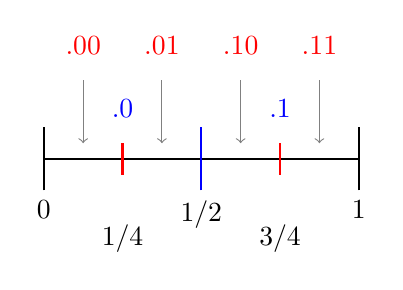
\begin{tikzpicture}[scale=4]
			% Eje principal
			\draw[thick] (0,0) -- (1,0);
			
			% Nivel 0 (0 y 1)
			\draw[thick] (0,-0.1) node[below] {$0$} -- (0,0.1);
			\draw[thick] (1,-0.1) node[below] {$1$} -- (1,0.1);
			
			% Nivel 1 (Mitades)
			\draw[thick, blue] (0.5,-0.1) node[below, text=black] {$1/2$} -- (0.5,0.1);
			\node[above, blue] at (0.25, 0.1) {$.0$};
			\node[above, blue] at (0.75, 0.1) {$.1$};
			
			% Nivel 2 (Cuartos)
			\draw[thick, red] (0.25,-0.05) node[below, text=black, yshift=-0.5cm] {$1/4$} -- (0.25,0.05);
			\draw[thick, red] (0.75,-0.05) node[below, text=black, yshift=-0.5cm] {$3/4$} -- (0.75,0.05);
			\node[above, red] at (0.125, 0.3) {$.00$};
			\node[above, red] at (0.375, 0.3) {$.01$};
			\node[above, red] at (0.625, 0.3) {$.10$};
			\node[above, red] at (0.875, 0.3) {$.11$};
			
			% Conectores para mostrar pertenencia a subintervalos
			\draw[->, gray, thin] (0.125, 0.25) -- (0.125, 0.05);
			\draw[->, gray, thin] (0.375, 0.25) -- (0.375, 0.05);
			\draw[->, gray, thin] (0.625, 0.25) -- (0.625, 0.05);
			\draw[->, gray, thin] (0.875, 0.25) -- (0.875, 0.05);
		\end{tikzpicture}
		\caption{Interpretación de $h((x_n))$ como expansión binaria. Los dígitos de la sucesión $(x_0, x_1, \dots)$ especifican sucesivamente en qué mitad del intervalo cae el punto.}
		\label{fig:expansion_binaria}
	\end{figure}
	
	Comprobamos la condición de semiconjugación $h \circ \sigma = f \circ h$:
	\begin{align*}
		h(\sigma(x_0, x_1, x_2 \dots)) &= h(x_1, x_2, \dots) = \sum_{n=0}^{\infty} \frac{x_{n+1}}{2^{n+1}} \\
		f(h(x_0, x_1, \dots)) &= 2 \left( \sum_{n=0}^{\infty} \frac{x_n}{2^{n+1}} \right) \pmod 1 \\
		&= \left( x_0 + \sum_{n=1}^{\infty} \frac{x_n}{2^n} \right) \pmod 1
	\end{align*}
	Como $x_0 \in \{0,1\}$, al aplicar módulo 1 la parte entera desaparece, quedando exactamente la misma suma que obtuvimos para $h(\sigma(x))$. Así, la dinámica del shift sobre símbolos emula la dinámica de $2x \pmod 1$.
\end{ejemplo}

\begin{ejercicio}
	Muestre que si $f$ es topológicamente transitiva y $g$ es un factor de $f$ (es decir, existe una semiconjugación $h$), entonces $g$ también es topológicamente transitiva.
\end{ejercicio}
\begin{proof}[Solución]
	Sea $h: X \to Y$ la semiconjugación sobreyectiva y continua ($h \circ f = g \circ h$). Como $f$ es transitiva, existe un punto $x \in X$ con órbita densa, es decir $\overline{\mathcal{O}_f^+(x)} = X$.
	Queremos evaluar la órbita del punto $y = h(x)$ bajo la función $g$.
	Aplicando $h$ a la órbita densa, por continuidad de $h$ tenemos:
	$$h\left(\overline{\mathcal{O}_f^+(x)}\right) \subseteq \overline{h(\mathcal{O}_f^+(x))}$$
	Reemplazando la clausura en la izquierda, $h(X) \subseteq \overline{h(\mathcal{O}_f^+(x))}$. Por ser $h$ sobreyectiva, $h(X) = Y$.
	Además, evaluemos los puntos de la órbita mapeada:
	$h(f^n(x)) = g^n(h(x)) = g^n(y)$.
	Sustituyendo esto, obtenemos que $Y \subseteq \overline{\{g^n(y)\}_{n \ge 0}} = \overline{\mathcal{O}_g^+(y)}$.
	Como el espacio entero $Y$ está contenido en la clausura de la órbita de $y$, dicha órbita es densa, lo que demuestra que $g$ es topológicamente transitiva.
\end{proof}

% =========================================================================
% --- FIN INPUT SEMANA 3 ---
% =========================================================================